\documentclass{article}\usepackage[]{graphicx}\usepackage[]{color}
%% maxwidth is the original width if it is less than linewidth
%% otherwise use linewidth (to make sure the graphics do not exceed the margin)
\makeatletter
\def\maxwidth{ %
  \ifdim\Gin@nat@width>\linewidth
    \linewidth
  \else
    \Gin@nat@width
  \fi
}
\makeatother

\definecolor{fgcolor}{rgb}{0.345, 0.345, 0.345}
\newcommand{\hlnum}[1]{\textcolor[rgb]{0.686,0.059,0.569}{#1}}%
\newcommand{\hlstr}[1]{\textcolor[rgb]{0.192,0.494,0.8}{#1}}%
\newcommand{\hlcom}[1]{\textcolor[rgb]{0.678,0.584,0.686}{\textit{#1}}}%
\newcommand{\hlopt}[1]{\textcolor[rgb]{0,0,0}{#1}}%
\newcommand{\hlstd}[1]{\textcolor[rgb]{0.345,0.345,0.345}{#1}}%
\newcommand{\hlkwa}[1]{\textcolor[rgb]{0.161,0.373,0.58}{\textbf{#1}}}%
\newcommand{\hlkwb}[1]{\textcolor[rgb]{0.69,0.353,0.396}{#1}}%
\newcommand{\hlkwc}[1]{\textcolor[rgb]{0.333,0.667,0.333}{#1}}%
\newcommand{\hlkwd}[1]{\textcolor[rgb]{0.737,0.353,0.396}{\textbf{#1}}}%
\let\hlipl\hlkwb

\usepackage{framed}
\makeatletter
\newenvironment{kframe}{%
 \def\at@end@of@kframe{}%
 \ifinner\ifhmode%
  \def\at@end@of@kframe{\end{minipage}}%
  \begin{minipage}{\columnwidth}%
 \fi\fi%
 \def\FrameCommand##1{\hskip\@totalleftmargin \hskip-\fboxsep
 \colorbox{shadecolor}{##1}\hskip-\fboxsep
     % There is no \\@totalrightmargin, so:
     \hskip-\linewidth \hskip-\@totalleftmargin \hskip\columnwidth}%
 \MakeFramed {\advance\hsize-\width
   \@totalleftmargin\z@ \linewidth\hsize
   \@setminipage}}%
 {\par\unskip\endMakeFramed%
 \at@end@of@kframe}
\makeatother

\definecolor{shadecolor}{rgb}{.97, .97, .97}
\definecolor{messagecolor}{rgb}{0, 0, 0}
\definecolor{warningcolor}{rgb}{1, 0, 1}
\definecolor{errorcolor}{rgb}{1, 0, 0}
\newenvironment{knitrout}{}{} % an empty environment to be redefined in TeX

\usepackage{alltt}
\usepackage[letterpaper, total={6in, 8in}]{geometry} %size of paper
\usepackage{indentfirst} %indent after section 
\usepackage{graphicx}
\usepackage{amsmath} %number figure based on subsection also
\numberwithin{figure}{subsection} %number figure based on subsection also
\numberwithin{table}{subsection} %number table based on subsection also
\bibliographystyle{plainnat} %for reference, but seems not work 
\usepackage{caption}%trick on caption
\captionsetup[figure]{labelfont=bf}
\captionsetup[table]{labelfont=bf,position=below}

\setlength{\parindent}{8ex}
\setlength{\parskip}{2em}
\renewcommand{\baselinestretch}{2.0}

\title{\vspace{-5ex} Analysis of Size-biased Mitochondria Data \vspace{-2ex}}
\author{Yin-Ting Chou \\
  Advisor: Aaron Rendahl \vspace{-2ex}} 
\date{May 2nd 2017}

%%%%%%%%%%%%%%%%%%%%%%%%%%%%%%%%%%%%%%%%%%%%%%%%%%%%%%%%%%%%
\IfFileExists{upquote.sty}{\usepackage{upquote}}{}
\begin{document}
\maketitle

\begin{abstract}
The goal of this project is to find out whether properties (area, perimeter, circularity and aspect ratio) of mitochondria are different by locations (proximal end, middle and distal end) in a single muscle fiber cell from a young mouse. However, the observed data is not a random sample but a size-biased sample, so the Arithmetic Mean is biased as an estimator for population mean. I instead use the concept of the Weighted Distribution to explore both parametric and nonparametric estimators of the population mean in the case of a size-biased sample. I first did a simulation study, which confirmed that arithmetic mean was inappropriate but that estimators based on the weighted distribution were appropriate with the parametric version having more assumptions but smaller standard deviation. I then applied these estimators in a Permutation Test, and constructed Bootstrapped confidence intervals for the parameters. I found mitochondria at the Middle have significantly larger Area and Perimeter and ones close to Distal end have significantly smaller Area, Perimeter and Circularity. Although the data in this project is from a single muscle fiber cell, the analysis results provide a strong foundation for future research on more cells.  
\end{abstract}

\newpage
[Intentionally blank page]
\newpage

\section{Introduction} 
This thesis is an extended study of my summer statistical consulting project which I worked in a pair with a PhD student, Ming Guo, at the Statistical Consulting Center in 2015. The client for this project was Professor Arriaga, the head of the Organelle Research Group in the University of Minnesota. The mission of his group is to answer complex questions related to the aging process, diabetes, obesity and neurodegeneration by starting with single cell and subcellular studies. This project is a preliminary study about the aging process and the main goal of this project is to understand whether properties (area, perimeter, circularity and aspect ratio) of mitochondria are different by locations (proximal, middle and distal end) in a single muscle fiber cell from a young mouse. After the main question is answered in this one cell, Prof.\ Arriaga team will start to test on many other cells. So, a secondary goal is to evaluate this data collecting procedure and provide suggestions on sampling methods. Due to the relationship between mitochondria and cell aging, the results of this project may be crucial to future research on the aging process, as described by Bratic and Larsson (2013).
 
The data of this project was collected by using the Transmission Electron Microscopy (TEM) technique to obtain super-resolution images of the single muscle fiber cell and then to manually measure properties (perimeter, area, circularity and aspect ratio) of sampled mitochondria from these images. Instead of choosing samples by using simple random sampling method, the sampled mitochondria were chosen if their area in the photo included one or more generated two-dimensional coordinates. A list of random coordinates was generated at the beginning of the sampling procedure. As a result of this procedure, each mitochondrion in the cell had a different probability of being picked as the sample and its sampling probability was proportional to its size (PPS), or its Area in this case. In this situation, if Arithmetic Mean was used as our estimator for the population mean Area, it would be overestimated even though it's widely used as the best estimator for population mean. To deal with this problem, Cox (1962) first proposed the concept of the Weighted Distribution to adjust the current sampling density function when samples are size-biased rather than random, and then Patil and Ord (1976) further extended this concept on parametric distributions. 

To find out the appropriate estimator of population mean as samples are size-biased, a simulation study was employed to test performance of the candidate estimators based on the selecting criteria, Root of MSE. The candidate estimators for the population mean Area are Arithmetic Mean (AM), Weighted Mean (WM) and Maximum Likelihood Estimator (MLE). Though we already knew that Arithmetic Mean would be overestimated, we were still interested in how bad it can be compared to other estimators. I have tried to add one more estimator which was based on the idea of Jones (1991) about estimating Weighted Distribution by kernel density. However, the result of this estimator was so close to Weighted Mean that I decided to drop this estimator on the candidate list. As for Perimeter, as we can see in Figure~\ref{scatter}, Area and Perimeter had a strong positive relation which means that mitochondria with large size also have large perimeter. If mitochondria with larger size are more easily picked then it is also true to mitochondria with large perimeter. So, we can say Perimeter in this case is Area-biased. Hence, our candidate estimators for Perimeter mean are also not only Arithmetic Mean (AM), but also Weighted Mean (WM), Delta Method Estimator (DME) and 2nd Order Taylor's Approximation Estimator (2TAE), all of which consider the relationship between Area and Perimeter. For Circularity and Aspect Ratio, from Figure~\ref{scatter}, we found that mitochondria with larger Area do not mean to have larger Circularity and Aspect Ratio. In other words, though the mitochondria with larger size are more easily picked, it will not influence the random sampling process of Circularity and Aspect Ratio. That is, the samples of Circularity and Aspect Ratio can still be random samples under this size-biased sampling process. This case can also be explained as the following scenario. Suppose we have many different size of balls with number on them and the numbers are nothing to do with the size of balls. In this situation, even though the sampling probability of balls being picked is proportional to its size, the numbers on the chosen balls can still be treated as random numbers. Therefore, it is reasonable for us to use Arithmetic Mean (AM) as a reasonable estimator for the population means of Circularity and Aspect Ratio. 

After figuring out the best estimator for each property, I used these estimators to do hypothesis tests. Because of the violation of ANOVA assumption of normality, Permutation Test was used for the hypothesis test and Bootstrapping technique was also conducted for confidence intervals of mean properties and mean difference with Bonferroni Correction. In the end, a suggestion on sampling procedure for future study on many other cells was provided based on the findings in the simulation study. 

\bigbreak
\begin{figure}[!htbp]
  \centering
\begin{knitrout}
\definecolor{shadecolor}{rgb}{0.969, 0.969, 0.969}\color{fgcolor}
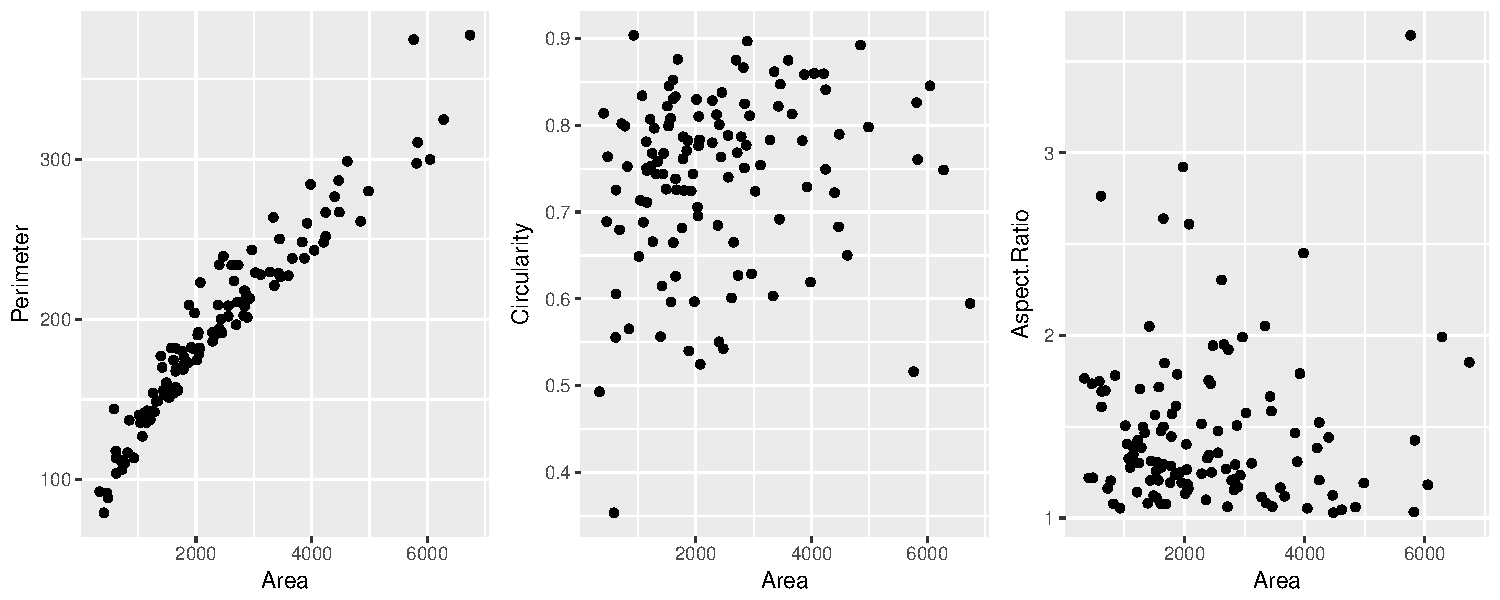
\includegraphics[width=\maxwidth]{figure/unnamed-chunk-1-1} 

\end{knitrout}
  \caption{Scatter plots for Area vs. Perimeter, Area vs. Circularity and Area vs. Aspect Ratio}
  \label{scatter}
\end{figure}

\newpage
[Intentionally blank page]
\newpage

\end{document}
